  \chapter{Многозадачные модели}\label{mtl} 

Многозадачное обучение - это метод разделения параметров между моделями, обучающимися выполнять несколько задач. Для нейронной сети его можно реализовать, приравняв значения разных слоев друг к другу.  В нейронных сетях это можно легко сделать, привязав веса разных слоев.  Идея многозадачного обучения была впервые предложена Каруаной в 1993 году \cite{Caruana_1997}. Для нейросетевых методов обработки текста оно впервые было применено в 2008 году Коллобером и Вестоном \cite{Collobert_Weston_2008}. В их модели справочные таблицы (или матрицы вложения слов) разделены между двумя моделями, обученными различным задачам, как показано на рисунке 5.
Использование общих параметров дает моделям возможность обмениваться информацией низкого уровня. Также Коллобер и Вестон в своей статьа выдвинули ряд идей (предобученные представления слов, исользование сверточных сетей), которые были по достоинству оценены позже - на конференции ICML 2018 получили награду "Испытание временем".


\begin{figure}[ht]
  \centerfloat{
    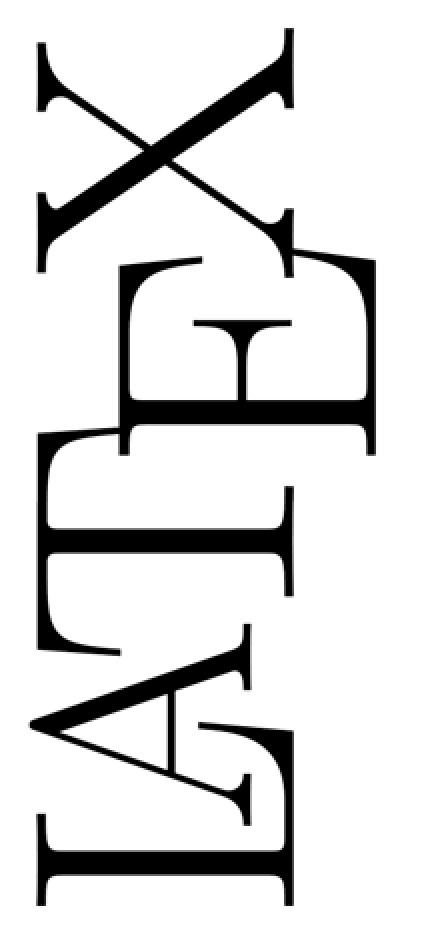
\includegraphics[scale=0.27]{latex}
  }
  \caption{Пример многозадачного обучения}\label{fig:MTL1}
\end{figure}

\section{Типы многозадачных архитектур}
Авторы обзора \cite{Chen_Zhang_Yang_2021} классифицировали архитектуры нейросетевых многозадачных моделей по следующим типам:
\begin{itemize}
\item[*] Параллельные архитектуры. Для данного типа архитектур одни и те же "общие" слои используются для примеров из каждой задачи, при этом выход "общих" слоев обрабатывается независимо своим специфическим слоем для каждой задачи. Плюсом данного типа архитектур является его достаточно высокая степень универсальности, а минусом - то, что необходимость получать одно и то же представление для каждой задачи может ограничивать адаптационные способности нейросетевой модели. К такому типу архитектур, в частности, принадлежит модель \textbf{MT-DNN} \cite{Liu_He_Chen_Gao_2019}, которая будет подробнее рассмотрена ниже. 
\item[*] Иерархические архитектуры. Для данного типа архитектур задачи обрабатываются зависимо друг от друга: так, результат классификации примера для одной из задач может использоваться при решении другой из задач как дополнительный входной параметр. Плюсом данного типа архитектур является возможность моделирования глубоких отношений между задачами, минусом - его негибкость. 
\item[*] Модульные архитектуры. Нейронная сеть в данных архитектурах делится на общие модули и задаче-специфичные модули, где общие модули имеют одни и те же веса для всех задач, а задаче-специфичные модули - свои веса для каждой из задач. Плюсом такого рода архитектур является возможность более "тонко" адаптировать модель для решения нескольких задач, что даёт возможность достигать высокой степени экономии вычислительных ресурсов и хороших результатов, реализованную, в частности, в статье \cite{Maziarka_Danel_2021}. Минусом же данного типа архитектур является отсутствие инвариантности по отношению к базовой модели : в отличие от параллельных архитектур, данный тип архитектур заточен под какую-то конкретную базовую нейросетевую модель, что делает замену базовой модели "под капотом" для многозадачных моделей из данного типа архитектур технически сложной. Данную архитектуру имеет, в частности, модель PAL-BERT  \cite{Stickland_Murray_2019}, которая будет рассмотрена в следующих разделах. 
\item[*] Генеративно-состязательные архитектуры. Для данного типа архитектур генератор и дискриминатор обучаются совместно таким образом, что дискриминатор пытается предсказать, из какой задачи пример, по его выдаваемому генератором представлению. А генератор, соответственно, пытается сгенерировать такое представление, чтобы дискриминатор мог предсказать задачу как можно хуже. Такое "состязание" генератора и дискриминатора даёт возможность генератору научиться выдавать представления примера, максимально инвариантные относительно задачи, которые в дальнейшем классифицируются скрытыми слоями на выходе, специфичными для каждой задачи. Подобный тип архитектур распространен достаточно мало в связи со своей негибкостью и нестабильностью обучения генеративно-состязательных сетей. Тем не менее, его неоспоримым преимуществом является возможность использовать большой объем неразмеченных данных для получения векторных представлений задач. 

В данной диссертационной работе исследовались возможности и особенности применения многозадачных нейросетевых моделей для обработки естественного языка. Был сделан упор на 2 нейросетевые архитектуры - модель MT-DNN \cite{Liu_He_Chen_Gao_2019} и модель PAL-BERT \cite{Stickland_Murray_2019}. Данные модели описаны подробнее в следующих разделах.

\section{Модель MT-DNN}
Модель MT-DNN - это многозадачная нейросетевая модель,которая относится к классу параллельных архитектурах. Данная модель, применяя один BERT к поступающему входу(с линейным pooling-слоем в конце), формирует на его базе свой собственный классификатор для каждой из задач. Модель делит все поступающие задачи на разные типы, включающие в себя, в частности:
\begin{itemize}
\item[*] Классификация текста. Пример - задачи CoLA, SST-2 из набора задач GLUE \cite{Wang_Singh_Michael_Hill_Levy_Bowman_2018}.
\item[*] Классификация пары последовательностей. Пример - задачи RTE, MNLI, QQP, MRPC из набора задач GLUE. 
\item[*] Задачи регрессии. Пример - задача STS-B из набора задач GLUE. 
\item[*] Задача попарного ранжирования ответов на вопросы. Авторы оригинальной статьи используют в этом качестве задачу QNLI из набора данных GLUE.
\item[*] Распознавание именованных сущностей. Пример - задача определения частей речи в наборе данных CONLL \cite{Erik F. Tjong Kim Sang_De Meulder_2003}. 
\end{itemize}

Модель принимает на вход последовательность токенов токенизированную способом, аналогичным описанному выше в разделе \textbf{Архитектура Трансформер и модель BERT} ССЫЛКА способу. Далее с данной последовательность происходят следующие трансформации:

\begin{itemize}
\item[*] Тренируемый слой L1 преобразует каждый токен в векторное представление, не зависящее от контекста. 
\item[*] Данное представление подается на вход кодировщику BERT, выходом которого является финальное векторное представление L2. 
\item[*] На выходе из L2 для каждого типа задач формируются задаче-специфичные слои, преобразующие это векторное представление и классифицирующие его. 
\end{itemize}
В общих чертах схема данной трансформации для набора данных GLUE приведена на рисунке. 

\begin{figure}[ht]
  \centerfloat{
    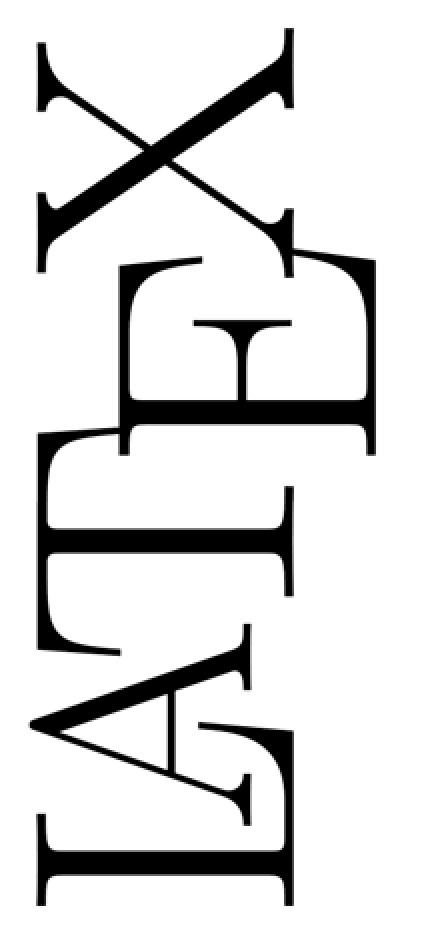
\includegraphics[scale=0.27]{latex}
  }
  \caption{Схема модели MT-DNN}\label{fig:MT-DNN1}
\end{figure}

В задаче-специфичных слоях для решения задачи классификации,вычисление  вероятности P(x) (вектор вероятностей P_{1},.... P_{n} для принадлежности к классу x_{1},... x_{n}) для векторного представления X токена [CLS] производится по формуле:
\begin{equation}
\color{black} P(x) = softmax(W^{T}X +B)  \label{eq:ref}
\end{equation}
где W^{T} матрица с тренируемыми коэффициентами размерности H*n, где H размерность скрытых состояний и n число классов, B тренируемый вектор размерности n
В качестве функции потерь для данной задачи используется кросс-энтропия. 

Для решения задачи определения семантической близости (такой, как STS-B) используется похожая формула:

\begin{equation}
\color{black} S(x) = W^{T}X +B \label{eq:ref}
\end{equation}

где W^{T} матрица тренируемых весовых коэффициентов размерности H*1, где H размерность скрытых состояний и 1 число классов, B тренируемый весовой коэффициент размерности 1. 
Близость S(x) может принимать значения от -\inf до \inf. В качестве функции потерь используется среднеквадратичная ошибка. 

Для задач классификации пары последовательностей в архитектуре MT-DNN используется стохастическая сеть ответов (stochastic answer network, SAN) \cite{Liu_Duh_Gao_2018}. Данная нейросетевая архитектура, основанная на рекуррентных слоях Gated Recurrent Unit(GRU)\cite{Cho_van Merrienboer_Bahdanau_Bengio_2014}, принимает на вход векторные представления пары последовательностей. На каждом шаге архитектура предсказывает возможные распределения вероятности между классами, что влияет на обновление весов модели. Финальные предсказанные вероятности получаются усреднением предсказанных вероятностей. 

Задача pairwise ranking (ранжирования пары последовательностей) решается аналогично предыдущим задачам, с соответствующими линейными трансформациями на входе и выходе.
Аналогичным же образом, с использованием линейных слоев, нейросетевая архитектура MT-DNN может быть адаптирована к решению задач распознавания именованных сущностей, что и было реализовано автором данной диссертационной работы в библиотеке DeepPavlov.

Как и оригинальный BERT, MT-DNN использует метод стохастического градиентного спуска для оптимизации функции потерь, подробнее описанный в \cite{Bousquet_Luxburg_Rätsch_2004}. На каждом этапе модель формирует батч B_{i} для решения целевой задачи i,   дообучая классификаторы и параметры BERT в соответствии со спецификой задачи. 

Авторы оригинальной статьи производили дообучение модели BERT в соответствии со следующими параметрами: скорость обучения 5*10^{-5}, оптимизатор Adamax \cite{Kingma_Ba_2014}, размер батча 32, 5 эпох. 

Как показано в оригинальной статье, несмотря на отсутствие адаптации под конкретную задачу, модель MT-DNN превосходит BERT-LARGE на всех задачах, кроме CoLA. Как показано в \cite{Коновалов_2022}, отставание на задаче CoLA связано с особенностями данного набора данных. 

Также в оригинальной статье показано, что, после дообучения на каждую конкретную задачу модель MT-DNN показывает дополнительный прирост качества; на задачах с ограниченной обучающей выборкой (MRPC, RTE, SST-2) прирост может достигать 1-2.5\%. Это говорит о том, что модель MT-DNN может переиспользовать свои знания, полученные при обучении на задачах  с более крупной обучающей выборкой, для решения задач с относительно маленькой выборкой.

Данные цифры показывают, что использование MT-DNN позволяет и экономить вычислительные ресурсы, и повышать при этом качество решения разных задач обработки естественного текста за счёт эффекта переноса знаний. 

Именно упрощенная модификация MT-DNN(без использования стохастических сетей ответов) использовалась в данной диссертационной работе и как трансформер-инвариантная нейросетевая архитектура, и как архитектура с одним линейным слоем, для которой исследовались различные варианты псевдоразметки данных. Подробнее данные исследования описаны в следующих главах. 

\section{Модель PAL-BERT}
Модель PAL-BERT, предложенная авторами статьи \cite{Stickland_Murray_2019}, представляет собой вариант модульной нейросетевой многозадачной архитектуры. У нейросетевой модели в данном варианте есть задаче-специфичные слои с весами, отдельными для каждой конкретной задачичи общие слои. При этом часть задаче-специфичных слоев встраивается непосредственно "в тело" модели, основанной на архитектуре Трансформер. 
Слои, встраиваемые "в тело" такой модели, называются PALs - Projective Attention Layers (проективные слои внимания). Их действие описывается формулой 

\begin{equation}
\color{black}PAL(h) = V_{d}*g(V_{e}*h) \label{eq:ref}
\end{equation}

где $V_{e$}$ матрица кодировщика размерности $S$*$H$, H размерность вектора скрытого слоя $$h$$, $S$<$H$ (авторы статьи предложили $S$=204 для BERT-LARGE), $V_{d}$ матрица декодировщика размерности $H$*$S$ и где g - многоголовое внимание.

Матрицы $V_{d}$ и $V_{e}$ одни и те же для каждого слоя, но специфичные для каждой конкретной задачи. 
Эти слои добавляются авторами данной нейросетевой архитектуры в модель BERT следующим образом. Если выход каждого следующего слоя стандартной модели BERT $BERT_{i}$ зависит от выхода предыдущего слоя $BERT_{i-1$ по формуле

\begin{equation}
\color{black}BERT_{i} =LayerNorm(BERT_{i-1})\label{eq:ref}
\end{equation},

то для модели PAL-BERT зависимость имеет такой вид:

\begin{equation}
\color{black}BERT_{i} =LayerNorm(BERT_{i-1} + PAL(BERT_{i-1)\label{eq:ref}
\end{equation}

\begin{figure}[ht]
  \centerfloat{
    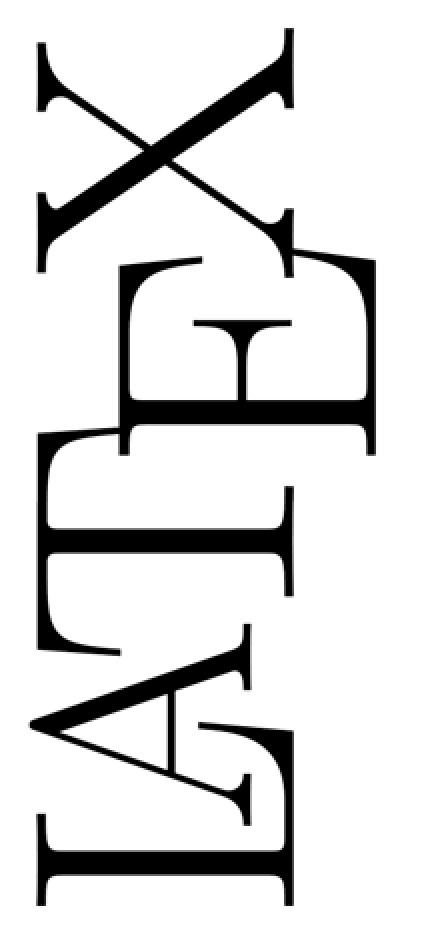
\includegraphics[scale=0.27]{latex}
  }
  \caption{ Использование проективных слоев внимания(PAL1, PAL2) в модели PAL-BERT. LN означает LayerNorm, SA самовнимание.}\label{fig:PAL1}
\end{figure}


Использование архитектуры PAL-BERT увеличивает число параметров, необходимых для решения 8 задач GLUE,всего на 13 процентов. 
Авторы оригинальной статьи также применяли многозадачное обучение для модели PAL-BERT с использованием аннеалированного сэмплирования (annealed sampling). При использовании данного типа сэмплирования, вероятность выбора примера из i-того задания P_{i} определяется следующим образом:

\begin{equation}
\color{black}P_{i} ~N^{(1-0.8*(e-1))/(E-1)}
\label{eq:ref}
\end{equation}
  
 где $e$ - номер эпохи, а $E$ - общее число эпох. 
Заметим, что полученные таким образом значения вероятностей нормируются на свою сумму. 
Как показано в оригинальной статье, модель PAL-BERT превосходит модель с добавлением одного линейного слоя "на верхушку" модели. В связи с хорошими показателями и низким вычислительным бюджетом, модель PAL-BERT применялась как многозадачная модель на одном из этапов развития диалоговой системы DREAM, о чем будет подробнее написано ниже. Однако отрицательным аспектом данной архитектуры является её негибкость и необходимость "вручную" подстраивать под каждую модификацию модели Transformer - а их на момент написания диссертации было разработано очень большое число, и регулярно появлялись новые модификации. В связи с необходимостью иметь возможность более "гибко" работать со всеми такими модификациями, было  принято решение в дальнейшем использовать иные имплементации многозадачных нейросетевых моделей в диалоговой системе DREAM. 
Обзор самой диалоговой системы DREAM приведён в следующем разделе. 

